\documentclass{standalone}
\usepackage{tikz}
\usetikzlibrary{patterns, positioning}


\begin{document}
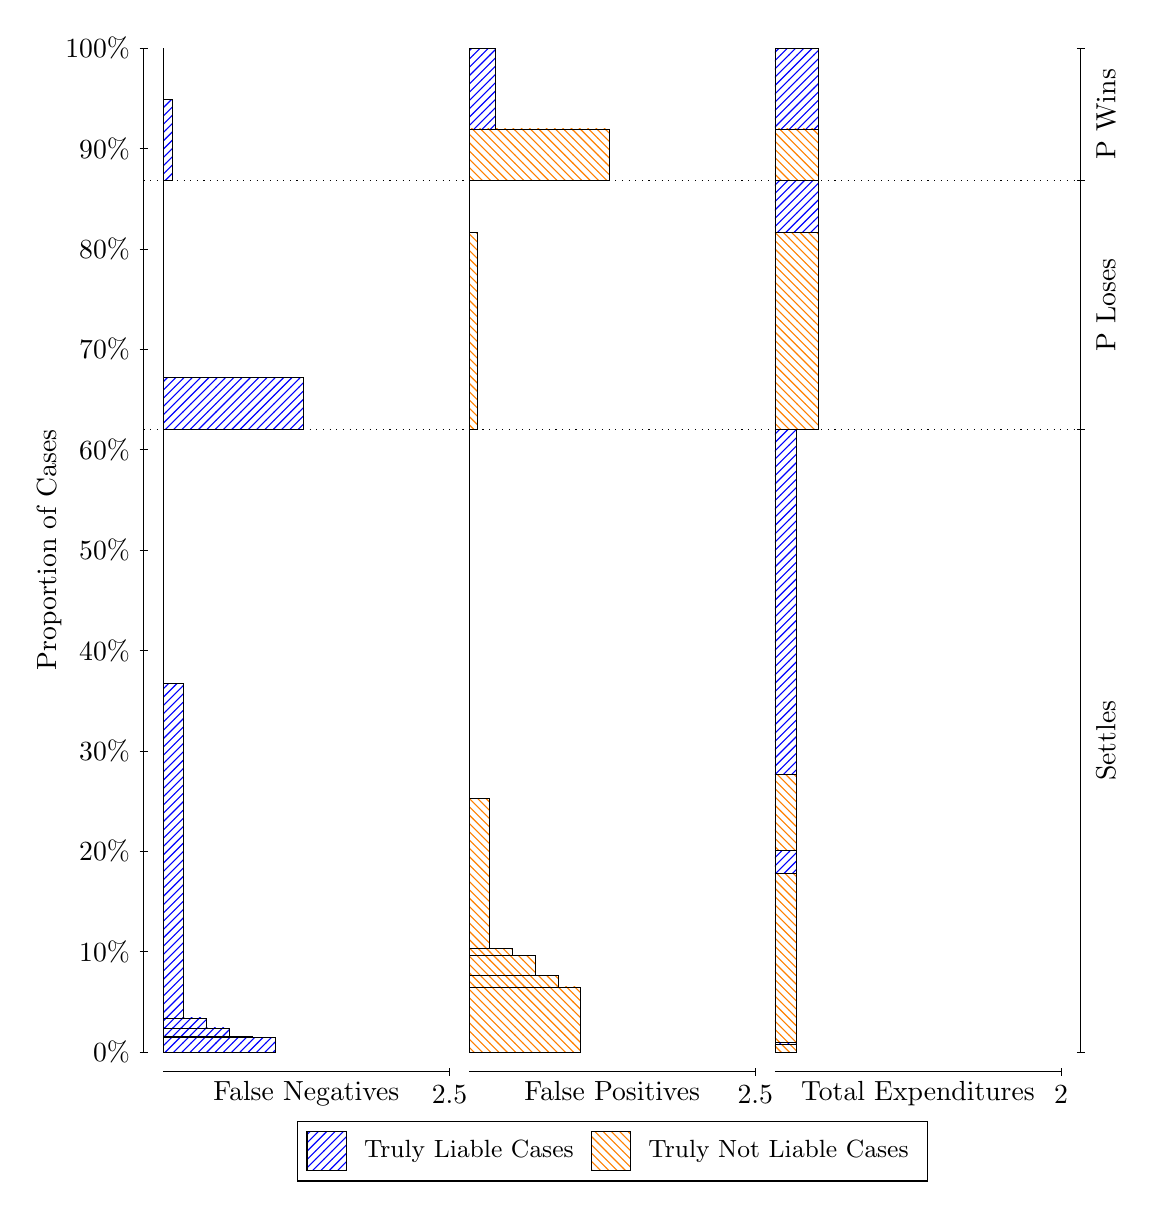
\begin{tikzpicture}
\draw[black, very thin] (1.5,1.75) -- (1.5,14.5);
\node[rotate=90, text=black, anchor=center] at (0.3, 8.125) {Proportion of Cases};
\draw[black, very thin] (1.45,1.75) -- (1.55,1.75);
\node[text=black, anchor=east] at (1.45, 1.75) {0\%};
\draw[black, very thin] (1.45,3.025) -- (1.55,3.025);
\node[text=black, anchor=east] at (1.45, 3.025) {10\%};
\draw[black, very thin] (1.45,4.3) -- (1.55,4.3);
\node[text=black, anchor=east] at (1.45, 4.3) {20\%};
\draw[black, very thin] (1.45,5.575) -- (1.55,5.575);
\node[text=black, anchor=east] at (1.45, 5.575) {30\%};
\draw[black, very thin] (1.45,6.85) -- (1.55,6.85);
\node[text=black, anchor=east] at (1.45, 6.85) {40\%};
\draw[black, very thin] (1.45,8.125) -- (1.55,8.125);
\node[text=black, anchor=east] at (1.45, 8.125) {50\%};
\draw[black, very thin] (1.45,9.4) -- (1.55,9.4);
\node[text=black, anchor=east] at (1.45, 9.4) {60\%};
\draw[black, very thin] (1.45,10.675) -- (1.55,10.675);
\node[text=black, anchor=east] at (1.45, 10.675) {70\%};
\draw[black, very thin] (1.45,11.95) -- (1.55,11.95);
\node[text=black, anchor=east] at (1.45, 11.95) {80\%};
\draw[black, very thin] (1.45,13.225) -- (1.55,13.225);
\node[text=black, anchor=east] at (1.45, 13.225) {90\%};
\draw[black, very thin] (1.45,14.5) -- (1.55,14.5);
\node[text=black, anchor=east] at (1.45, 14.5) {100\%};

\draw[black, very thin] (13.4,1.75) -- (13.4,14.5);
\draw[black, very thin] (13.35,1.75) -- (13.45,1.75);
\node[anchor=west] at (13.35, 1.75) {};
\draw[black, very thin] (13.35,9.6584) -- (13.45,9.6584);
\node[anchor=west] at (13.35, 9.6584) {};
\draw[black, very thin] (13.35,12.818) -- (13.45,12.818);
\node[anchor=west] at (13.35, 12.818) {};
\draw[black, very thin] (13.35,14.5) -- (13.45,14.5);
\node[anchor=west] at (13.35, 14.5) {};

\draw[black, very thin, pattern color=blue, pattern=north east lines] (1.75,1.75) rectangle (3.167,1.9309);
\draw[black, very thin, pattern color=blue, pattern=north east lines] (1.75,1.9309) rectangle (2.8763,1.9513);
\draw[black, very thin, pattern color=blue, pattern=north east lines] (1.75,1.9513) rectangle (2.5857,2.0573);
\draw[black, very thin, pattern color=blue, pattern=north east lines] (1.75,2.0573) rectangle (2.295,2.1831);
\draw[black, very thin, pattern color=blue, pattern=north east lines] (1.75,2.1831) rectangle (2.0043,6.4359);
\draw[black, very thin, pattern color=orange, pattern=north west lines] (1.75,6.4359) rectangle (1.75,9.6584);
\draw[black, very thin, pattern color=blue, pattern=north east lines] (1.75,9.6584) rectangle (3.5303,10.319);
\draw[black, very thin, pattern color=orange, pattern=north west lines] (1.75,10.319) rectangle (1.75,12.818);
\draw[black, very thin, pattern color=blue, pattern=north east lines] (1.75,12.818) rectangle (1.859,13.846);
\draw[black, very thin, pattern color=orange, pattern=north west lines] (1.75,13.846) rectangle (1.75,14.5);
\draw[black, very thin, pattern color=orange, pattern=north west lines] (5.6333,1.75) rectangle (7.0503,2.577);
\draw[black, very thin, pattern color=orange, pattern=north west lines] (5.6333,2.577) rectangle (6.7597,2.7222);
\draw[black, very thin, pattern color=orange, pattern=north west lines] (5.6333,2.7222) rectangle (6.469,2.973);
\draw[black, very thin, pattern color=orange, pattern=north west lines] (5.6333,2.973) rectangle (6.1783,3.0703);
\draw[black, very thin, pattern color=orange, pattern=north west lines] (5.6333,3.0703) rectangle (5.8877,4.9725);
\draw[black, very thin, pattern color=blue, pattern=north east lines] (5.6333,4.9725) rectangle (5.6333,9.6584);
\draw[black, very thin, pattern color=orange, pattern=north west lines] (5.6333,9.6584) rectangle (5.7423,12.157);
\draw[black, very thin, pattern color=blue, pattern=north east lines] (5.6333,12.157) rectangle (5.6333,12.818);
\draw[black, very thin, pattern color=orange, pattern=north west lines] (5.6333,12.818) rectangle (7.4137,13.472);
\draw[black, very thin, pattern color=blue, pattern=north east lines] (5.6333,13.472) rectangle (5.9603,14.5);
\draw[black, very thin, pattern color=orange, pattern=north west lines] (9.5167,1.75) rectangle (9.7892,1.8473);
\draw[black, very thin, pattern color=blue, pattern=north east lines] (9.5167,1.8473) rectangle (9.7892,1.8678);
\draw[black, very thin, pattern color=orange, pattern=north west lines] (9.5167,1.8678) rectangle (9.7892,4.0207);
\draw[black, very thin, pattern color=blue, pattern=north east lines] (9.5167,4.0207) rectangle (9.7892,4.3076);
\draw[black, very thin, pattern color=orange, pattern=north west lines] (9.5167,4.3076) rectangle (9.7892,5.2798);
\draw[black, very thin, pattern color=blue, pattern=north east lines] (9.5167,5.2798) rectangle (9.7892,9.6584);
\draw[black, very thin, pattern color=orange, pattern=north west lines] (9.5167,9.6584) rectangle (10.062,12.157);
\draw[black, very thin, pattern color=blue, pattern=north east lines] (9.5167,12.157) rectangle (10.062,12.818);
\draw[black, very thin, pattern color=orange, pattern=north west lines] (9.5167,12.818) rectangle (10.062,13.472);
\draw[black, very thin, pattern color=blue, pattern=north east lines] (9.5167,13.472) rectangle (10.062,14.5);
\draw[black, dotted] (1.5,9.6584) -- (13.4,9.6584);
\draw[black, dotted] (1.5,12.818) -- (13.4,12.818);
\draw[black, very thin] (1.75,1.5) -- (5.3833,1.5);
\node[text=black, anchor=north] at (3.5667, 1.5) {False Negatives};
\draw[black, very thin] (5.3833,1.45) -- (5.3833,1.55);
\node[text=black, anchor=north] at (5.3833, 1.45) {2.5};

\draw[black, very thin] (5.6333,1.5) -- (9.2667,1.5);
\node[text=black, anchor=north] at (7.45, 1.5) {False Positives};
\draw[black, very thin] (9.2667,1.45) -- (9.2667,1.55);
\node[text=black, anchor=north] at (9.2667, 1.45) {2.5};

\draw[black, very thin] (9.5167,1.5) -- (13.15,1.5);
\node[text=black, anchor=north] at (11.333, 1.5) {Total Expenditures};
\draw[black, very thin] (13.15,1.45) -- (13.15,1.55);
\node[text=black, anchor=north] at (13.15, 1.45) {2};

\node[text=black, centered, rotate=90] at (13.72, 5.7042) {Settles};
\node[text=black, centered, rotate=90] at (13.72, 11.238) {P Loses};
\node[text=black, centered, rotate=90] at (13.72, 13.659) {P Wins};

\draw (7.449999999999999,1.5) node[draw=none] (baseCoordinate) {};
\begin{scope}[align=center]
        \matrix[scale=0.5, draw=black, below=0.5cm of baseCoordinate, nodes={draw}, column sep=0.1cm]{
            \node[rectangle, draw, minimum width=0.5cm, minimum height=0.5cm, pattern color=blue, pattern=north east lines] {}; &
            \node[draw=none, font=\small, text=black] (B) {Truly Liable Cases}; &
            \node[rectangle, draw, minimum width=0.5cm, minimum height=0.5cm, pattern color=orange, pattern=north west lines] {}; &
            \node[draw=none, font=\small, text=black] (B) {Truly Not Liable Cases}; \\
            };
\end{scope}

\end{tikzpicture}
\end{document}